\documentclass[12pt, letterpaper]{article}

\usepackage[utf8]{inputenc}
\usepackage[margin=1in]{geometry}
\usepackage{comment}
\usepackage{caption} % for table captions

\usepackage[shortlabels]{enumitem} % for (a) (b) (c) enumerate use [(a)] like so:
%\begin{enumerate}[(a)]
\usepackage{bm}%bold symbols in math mode
\usepackage{amsmath}%allows text in math mode e.g. \text{}

\usepackage{listings} % Typeset Python
%Here is an example of how to do that
%\begin{lstlisting}[language=Python, basicstyle=\tiny]
%#Here is some test Python
%def yay():
%    print("hi")
%\end{lstlisting}

\usepackage{graphicx} % for images
%\includegraphics{uploaded-file-name}

\usepackage{float} % supposedly will allow the use of [H] for table and figure positioning

\title{COSC 5010-03 Practical Machine Learning Fall 2023 Exploratory Data Analysis Report}
\author{Michael Elgin}
\date{November 13, 2023}

\begin{document}

\maketitle

\section{Introduction} %What problem are you solving, how are you going to solve it.

Exploratory data analysis is an important consideration before creating machine-learning models. It can affect the choice of model, the choice of features to prune, or whether samples should be modified or deleted. This report examines the charactersistic of the wine quality dataset\footnote{https://archive.ics.uci.edu/dataset/186/wine+quality}. The dataset explored is created by concatenating both the red and white wine datasets together. Later, the class distributions for each of red and white are individually examined.

\section{Analysis and its Results}

\subsection{Dataset Basics}

The dataset contains 11 features, all of which are real numbers. The quality (target) is an integer. There are a total of 6497 samples. There are no missing values. Approximately 75\% of the samples are white, and 25\% are red.

\subsection{Feature Correlations}

Feature correlations are an important facet of a dataset to explore. The first reason is that there are certain types of models, such as linear models, that expect features not to be correlated. If this is not the case, a linear model may end up assigning unpredictable and inaccurate weights to features. For example, if a linear model predicting circumference of circles is trained on radius as one feature \emph{and} diameter as the second, it may assign an arbitrary weight less than $2\pi$ to the radius and likewise an arbitrary weight less than $\pi$ to the diameter such that the weighted sum always arrives properly at the circumference. But of course in reality this is nonsense; as we know the weights should be \emph{exactly} $2\pi$ and $\pi$ respectively. The issue is correlation, in this case the logical extreme of perfect correlation. Knowing the second value provides no new information and merely creates weights that don't reflect how the feature truly influences the target in reality. The solution is to prune highly correlated features so only one is left.

The second reason is that there is a model-agnostic interpretability method known as partial dependence plots, which are made by creating artificial datasets by setting a feature to be a specific value for all samples, and then finding the model's average prediction for all those samples. Varying the value shows how model prediction changes accordingly (on average). The reason why correlated features are an issue here is that if a plotted feature is correlated with another (unplotted) feature, in reality it won't change by itself. Thus showing how one feature affects model output as it changes independently is misleading because it will never change independently from it's correlated feature. One may observe a change to the feature in the plot and think that the model will also change according to the plot, but it will not because that change in the original feature also involves a hidden change to the correlated feature which will affect model output some way; a way that the partial dependence plot doesn't account for.

Feature correlations are easily visualized by heatmaps. A common technique is to set positively correlated features to one color, negatively correlated features to the opposite color, and no correlations to white. This allows one to easily spot the most correlated features. The correlations for the wine quality dataset are shown in figure \ref{corr}.

\begin{figure}[H]
    \centering
    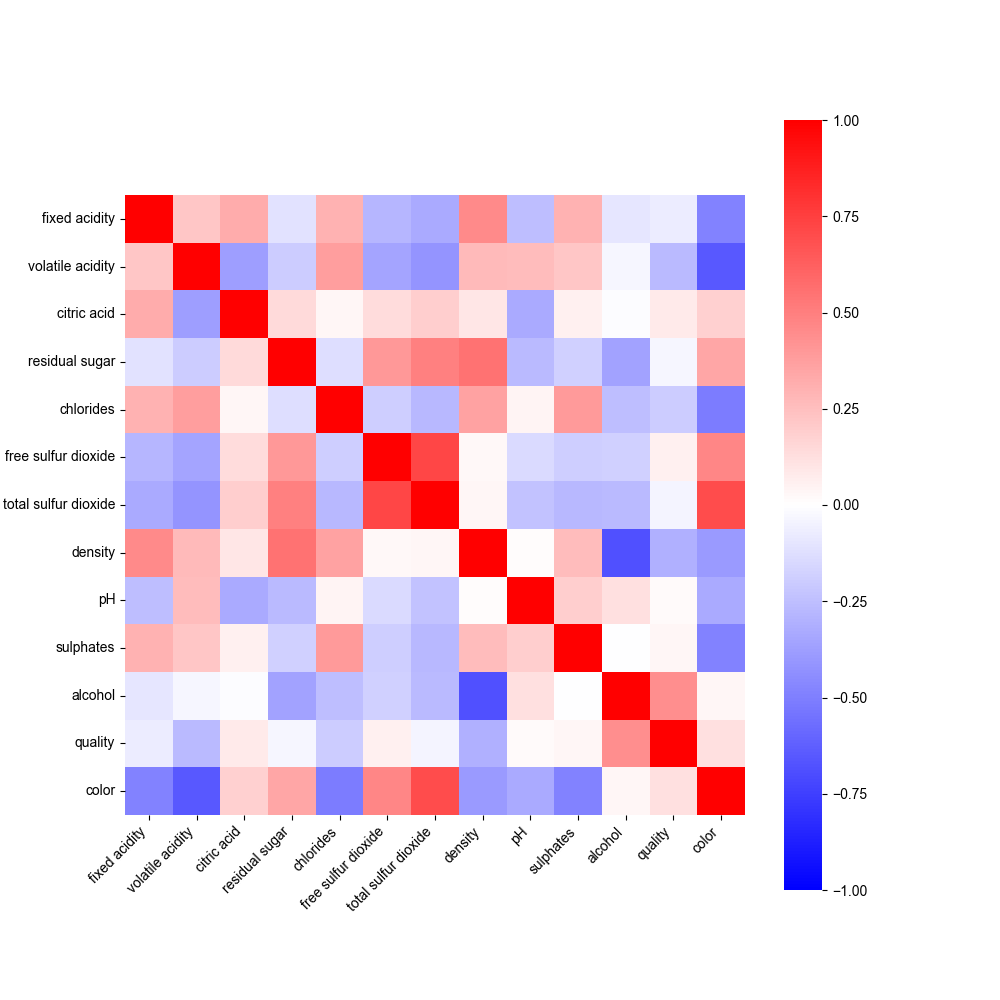
\includegraphics[scale=0.625]{correlations.png}
    \caption{Feature and target correlations}
    \label{corr} % For referencing the figure later in the document
\end{figure}

From here, one can spot free sulphur dioxide and total sulfur dioxide as highly correlated features. This is no surprise, for obvious reasons. At least one of the features should be pruned, most likely total sulfur dioxide. Likewise one can also spot the negative correlation between alcohol and density. This makes intuitive sense, since increasing the amount of alcohol (and thus decreasing water) is always going to change the density in the same direction.

A third reason to know the correlations is to see which features are correlated with the target, as this provides direct insight into which features are influential at changing the target and thus tell something to a model about what target to predict.

\subsection{Class Density Distributions}

\subsubsection{Concatenated Dataset}

An important part of exploratory data analysis involving continuous features and a classification target is to plot the density functions of each class along each feature in the same graph, to see how much separation a feature may give between the classes. This visually shows the differences in features between the classes.

\newcommand{\myscale}{.9775}
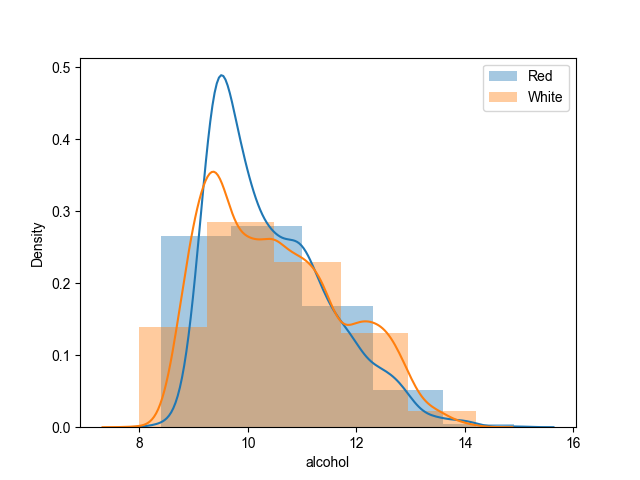
\includegraphics[scale=\myscale]{class_dist_alcohol.png}

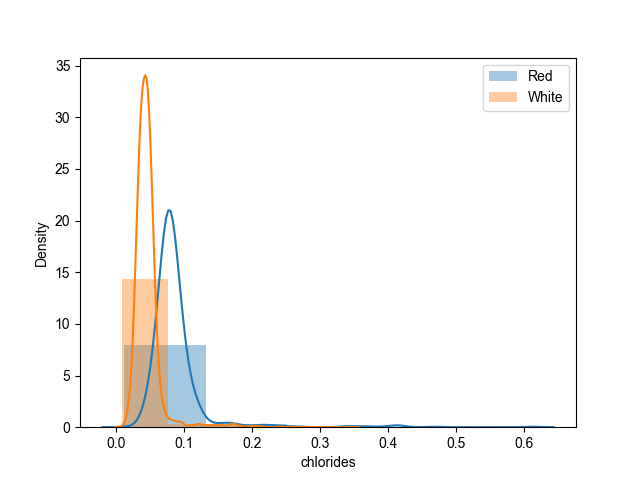
\includegraphics[scale=\myscale]{class_dist_chlorides.png}

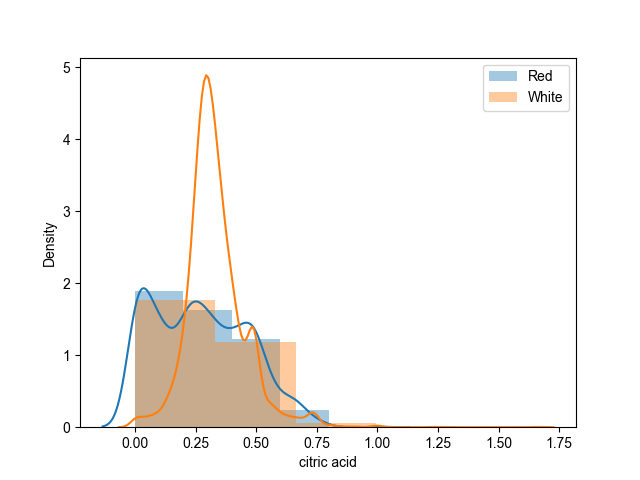
\includegraphics[scale=\myscale]{class_dist_citric_acid.png}

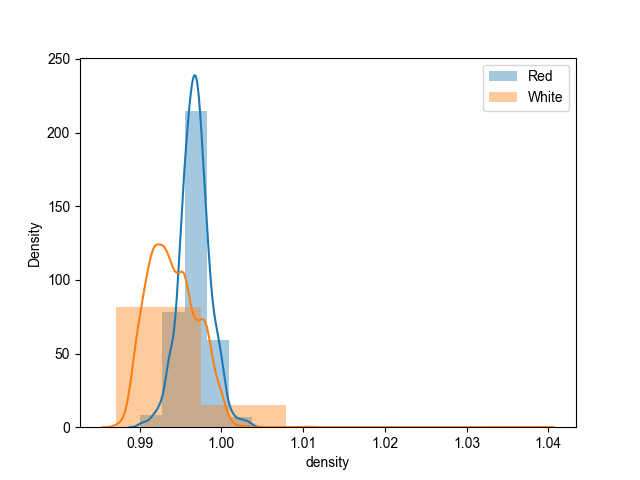
\includegraphics[scale=\myscale]{class_dist_density.png}

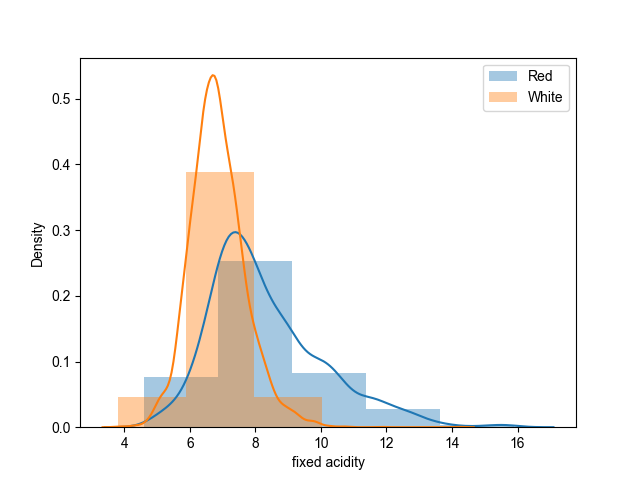
\includegraphics[scale=\myscale]{class_dist_fixed_acidity.png}

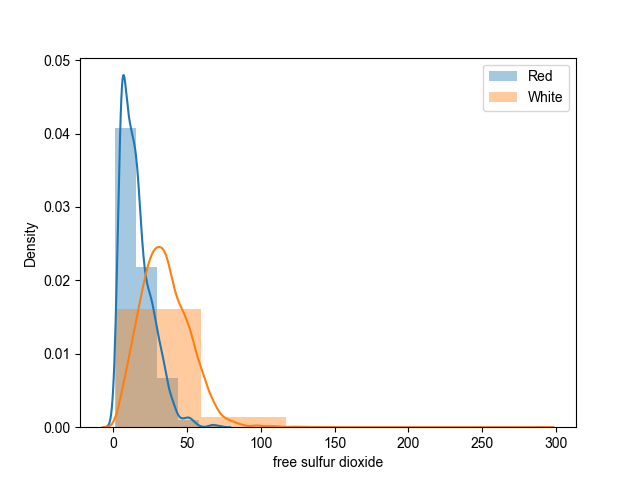
\includegraphics[scale=\myscale]{class_dist_free_sulfur_dioxide.png}

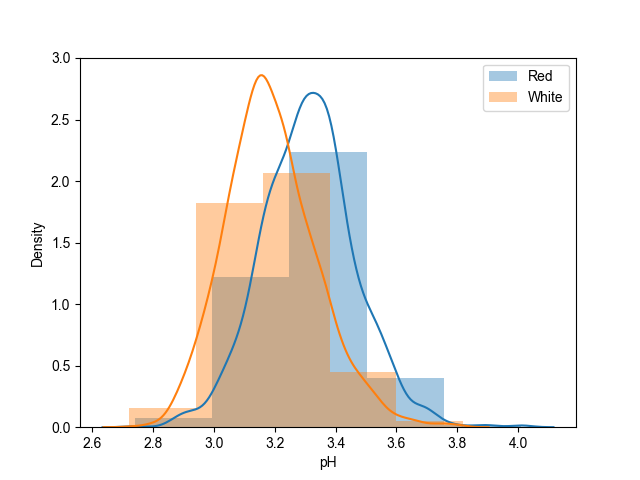
\includegraphics[scale=\myscale]{class_dist_pH.png}

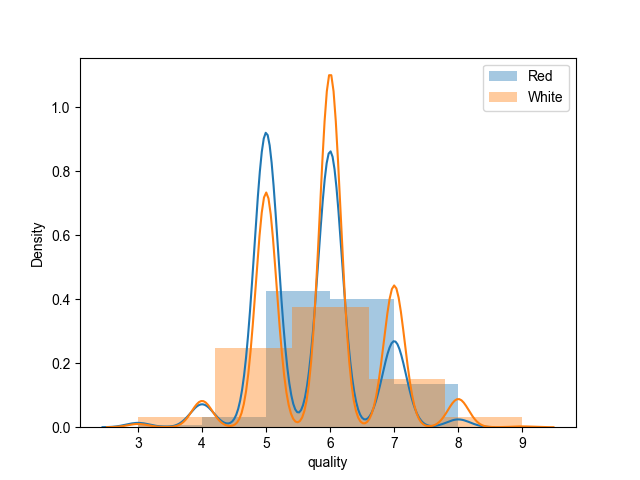
\includegraphics[scale=\myscale]{class_dist_quality.png}

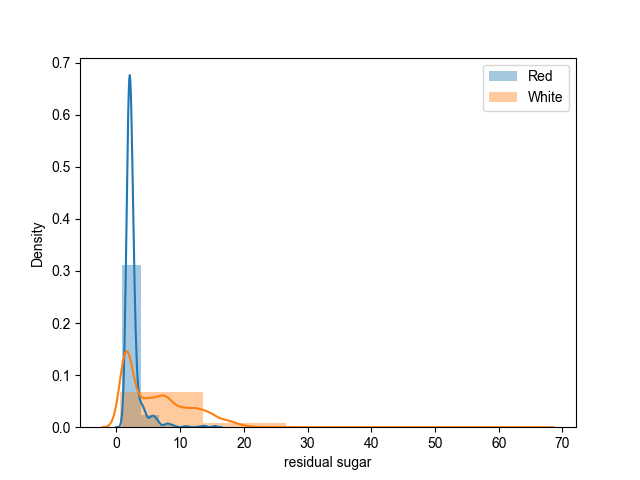
\includegraphics[scale=\myscale]{class_dist_residual_sugar.png}

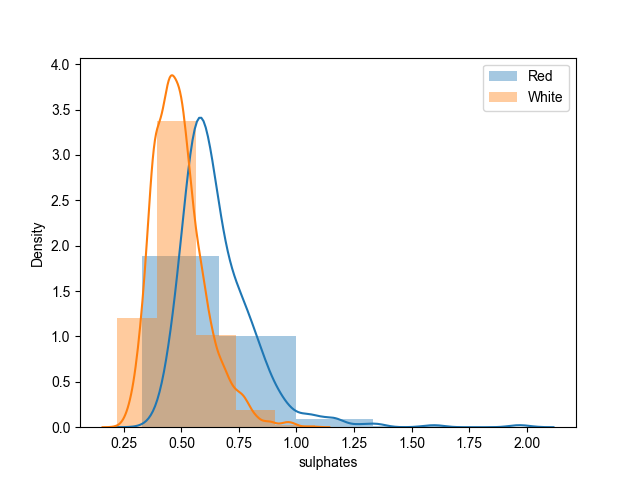
\includegraphics[scale=\myscale]{class_dist_sulphates.png}

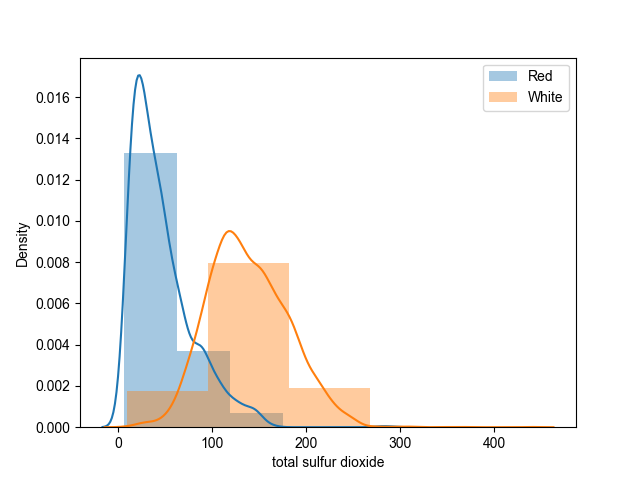
\includegraphics[scale=\myscale]{class_dist_total_sulfur_dioxide.png}

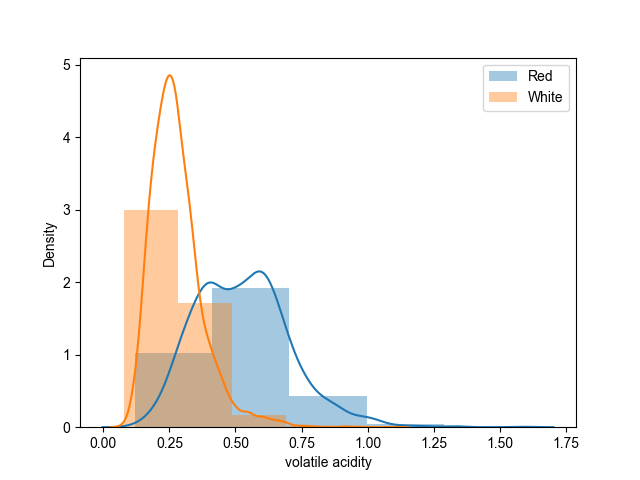
\includegraphics[scale=\myscale]{class_dist_volatile_acidity.png}

There is not complete separation given by any feature. However there is still some healthy separation in chlorides, volatile acidity, free sulfur dioxide, total sulfur dioxide, and residual sugar. These will be features that are likely to be of most use in classification.

\subsubsection{Red and White Datasets}

This section plots density functions for each color individually, to see which features may give good separation between quality levels. Red is examined first.

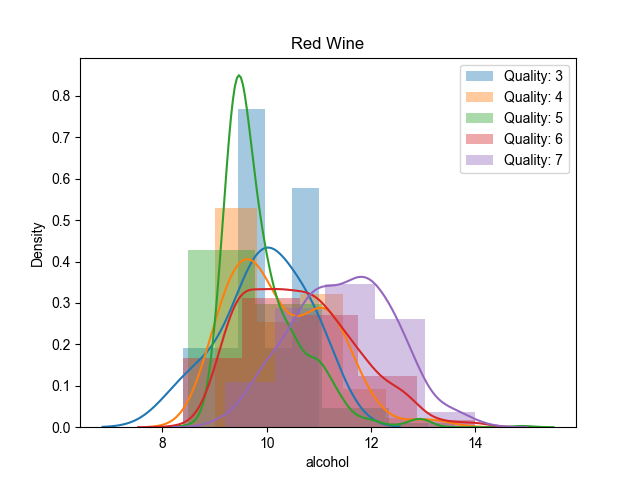
\includegraphics[scale=\myscale]{red_quality_dist_alcohol.png}

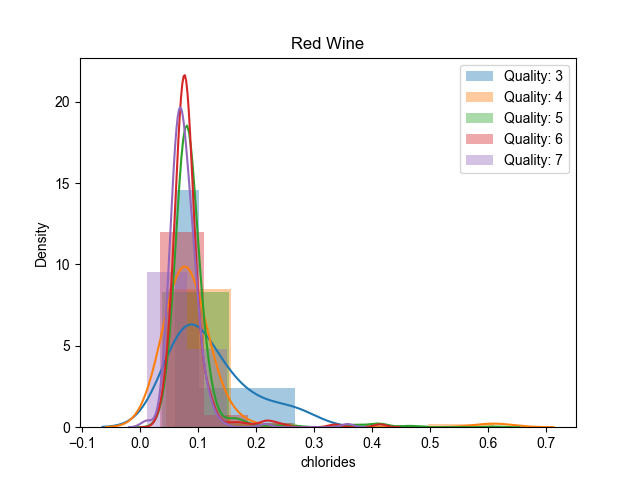
\includegraphics[scale=\myscale]{red_quality_dist_chlorides.png}

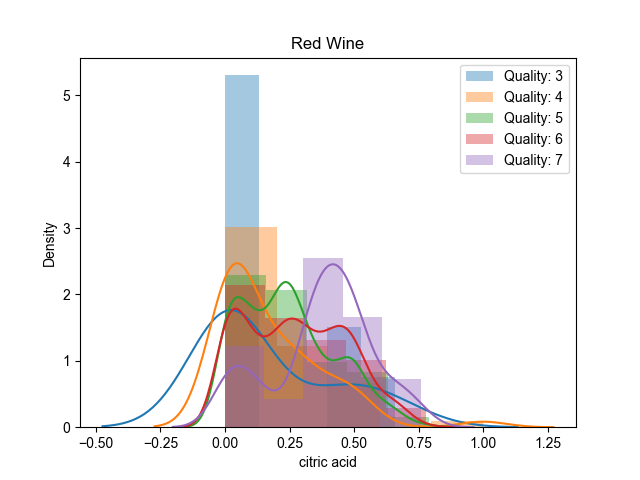
\includegraphics[scale=\myscale]{red_quality_dist_citric_acid.png}

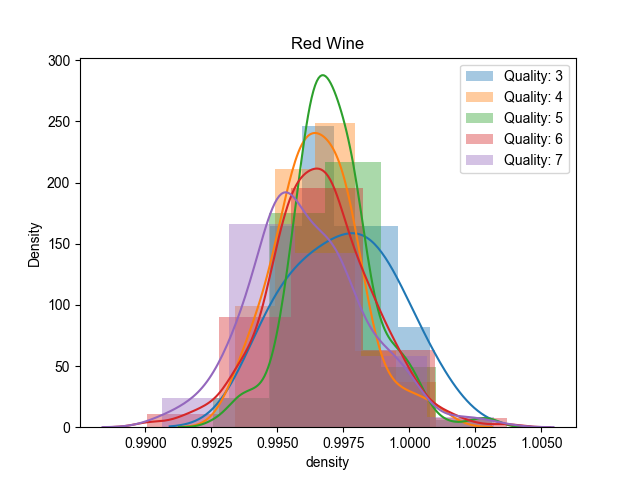
\includegraphics[scale=\myscale]{red_quality_dist_density.png}

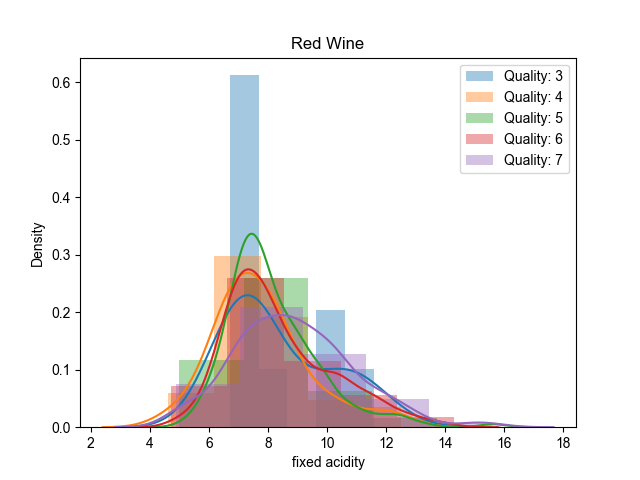
\includegraphics[scale=\myscale]{red_quality_dist_fixed_acidity.png}

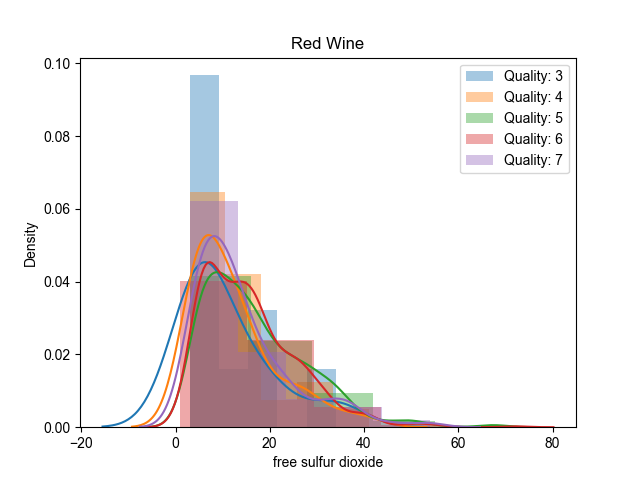
\includegraphics[scale=\myscale]{red_quality_dist_free_sulfur_dioxide.png}

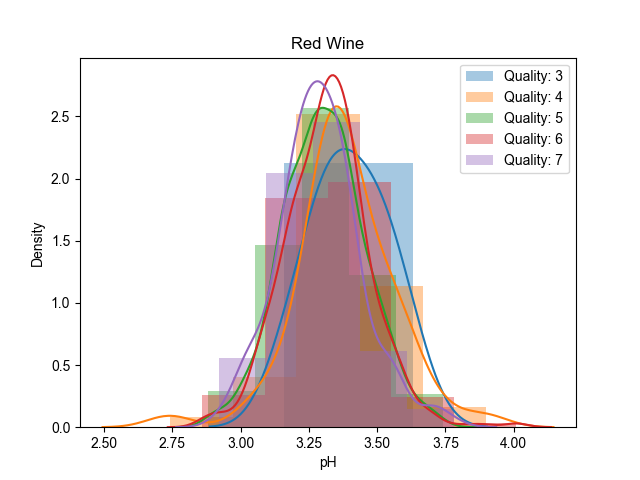
\includegraphics[scale=\myscale]{red_quality_dist_pH.png}

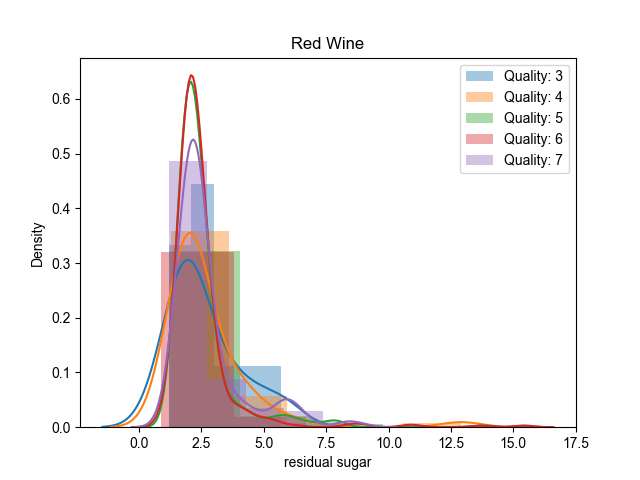
\includegraphics[scale=\myscale]{red_quality_dist_residual_sugar.png}

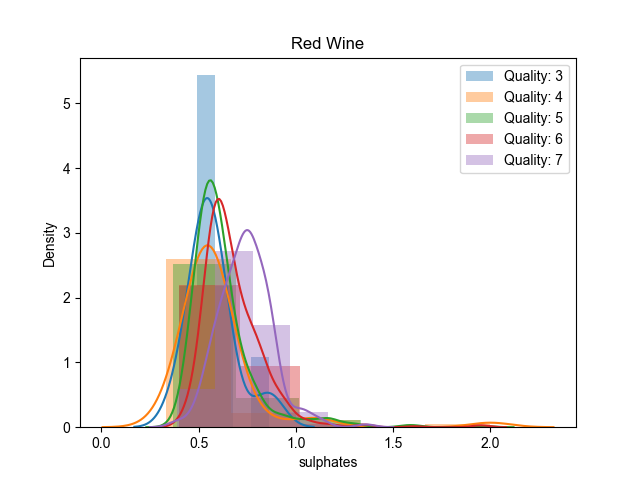
\includegraphics[scale=\myscale]{red_quality_dist_sulphates.png}

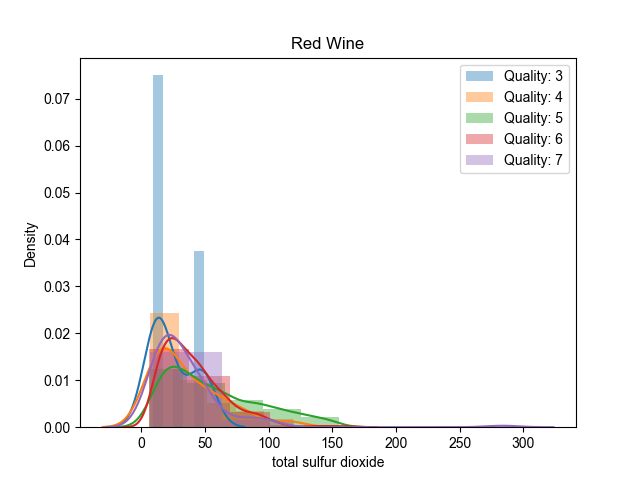
\includegraphics[scale=\myscale]{red_quality_dist_total_sulfur_dioxide.png}

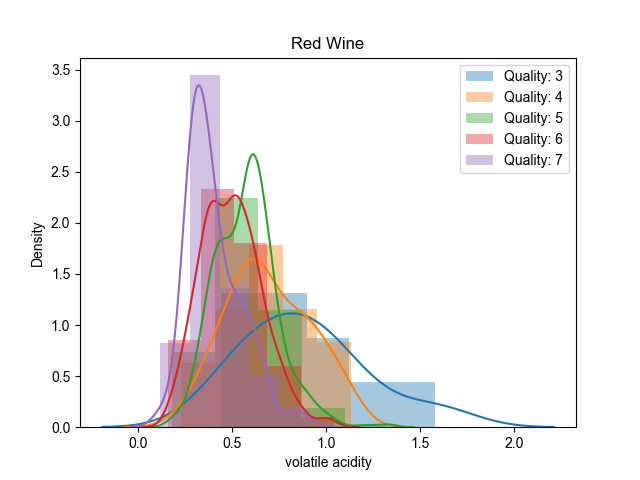
\includegraphics[scale=\myscale]{red_quality_dist_volatile_acidity.png}

What is most prominent is the difference between low quality wines (blue) and high quality wines (purple). Low quality wines tend to especially have low alcohol, citric acid, free/total sulfur dioxide, and high volatile acidity. High quality wines tend to have the opposite.

White wine is examined next.

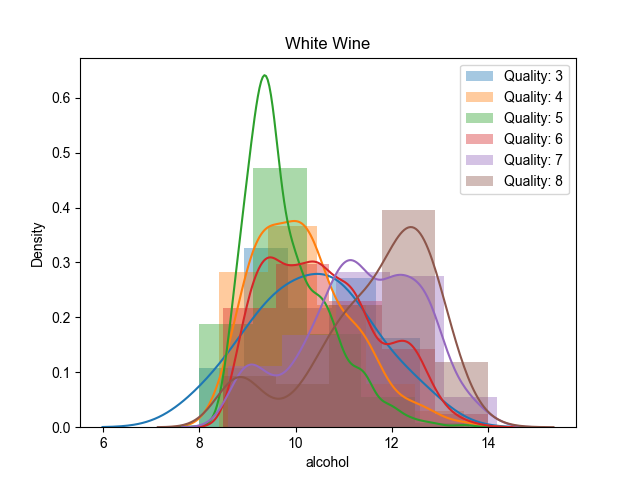
\includegraphics[scale=\myscale]{white_quality_dist_alcohol.png}

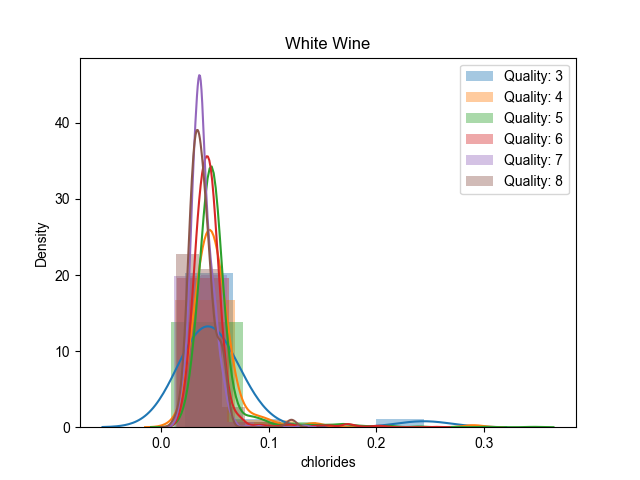
\includegraphics[scale=\myscale]{white_quality_dist_chlorides.png}

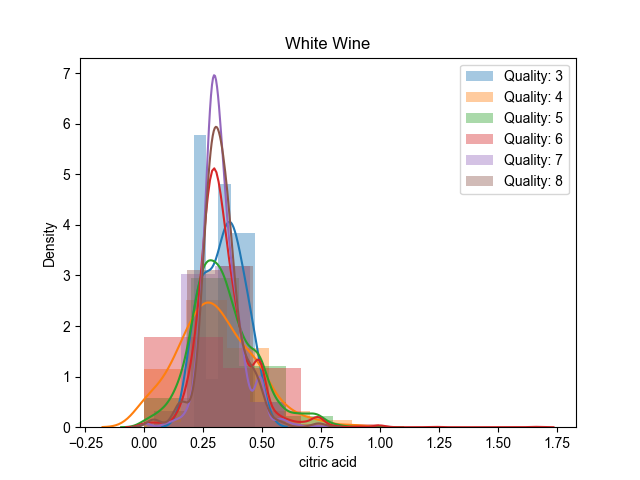
\includegraphics[scale=\myscale]{white_quality_dist_citric_acid.png}

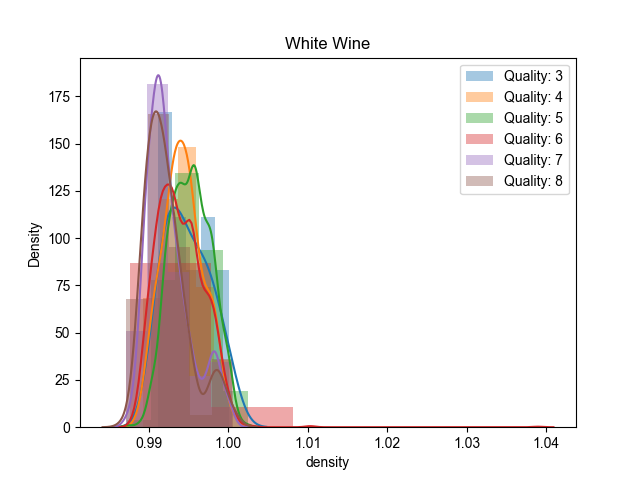
\includegraphics[scale=\myscale]{white_quality_dist_density.png}

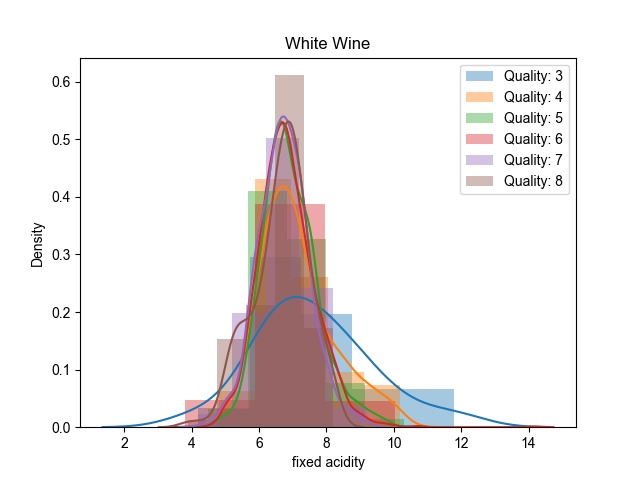
\includegraphics[scale=\myscale]{white_quality_dist_fixed_acidity.png}

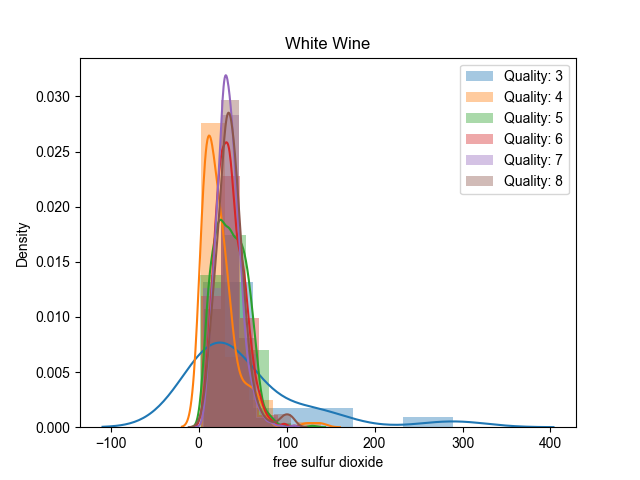
\includegraphics[scale=\myscale]{white_quality_dist_free_sulfur_dioxide.png}

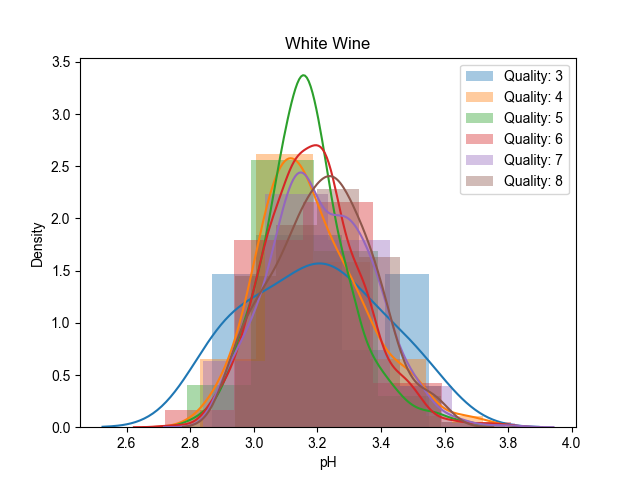
\includegraphics[scale=\myscale]{white_quality_dist_pH.png}

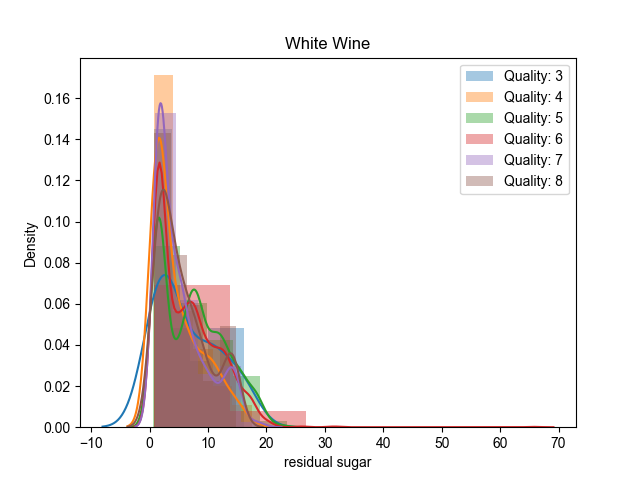
\includegraphics[scale=\myscale]{white_quality_dist_residual_sugar.png}

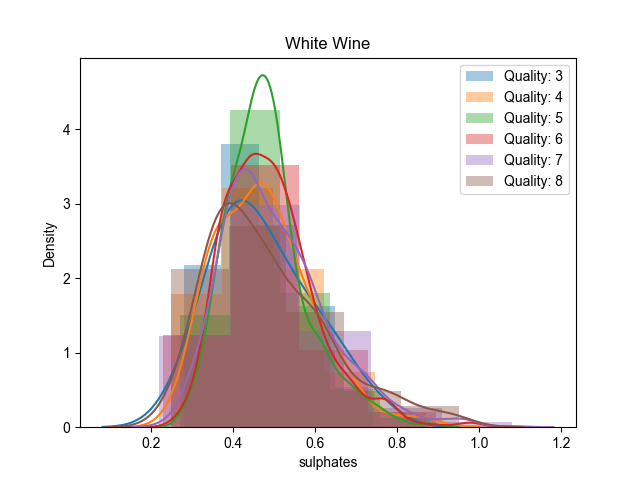
\includegraphics[scale=\myscale]{white_quality_dist_sulphates.png}

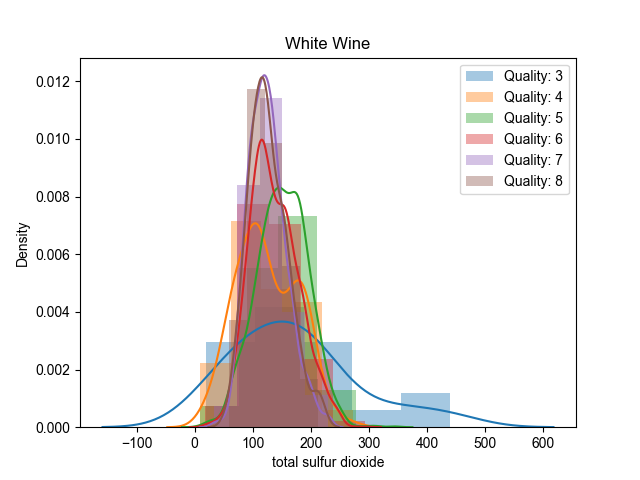
\includegraphics[scale=\myscale]{white_quality_dist_total_sulfur_dioxide.png}

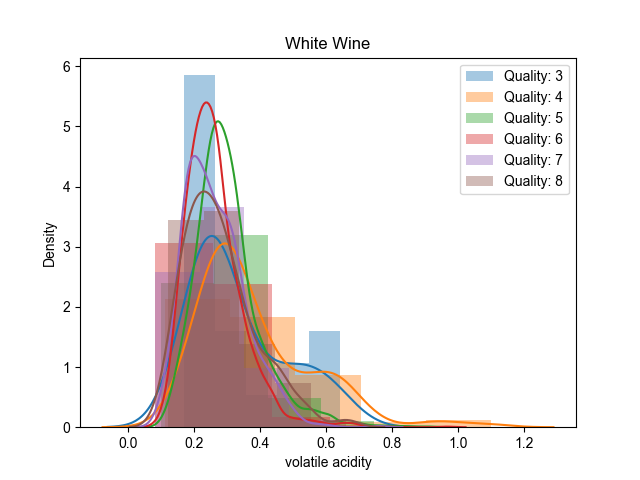
\includegraphics[scale=\myscale]{white_quality_dist_volatile_acidity.png}

For white, low quality wines tend to have high fixed acidity, high volatile acidity, high free/total sulfur dioxide.

\section{Code} %Add the code you've used as a separate file.

The associated code is in EDA.ipynb

\end{document}